This chapter describes how to simulate from our multiGLMM, and describes
a real-based dataset used as an application example. The simulation
procedure is addressed in \autoref{cap:simu}. In \autoref{cap:data} a
simulated dataset based on the Nordic Cancer Union (NCU) twins data is
presented as an application example.

\section{SIMULATING FROM THE MODEL}
\label{cap:simu}

Being able to simulate data from a model is a key task, fundamental to
assess the finite-sample properties and the estimation procedure
liability of a given statistical model. The step-by-step describing the
simulation procedure of our multiGLMM is presented on Algorithm
\autoref{alg:algo}, following the model hierarchical structure
stipulated in \autoref{eq:model}.

\begin{algorithm}[H]
 \caption{SIMULATING FROM A \(\text{multiGLMM}\) FOR CLUSTERED COMPETING
          RISKS DATA}
 \label{alg:algo}
 \begin{algorithmic}[1]
  \State
   Set \(J\), the number of clusters
  \State
   Set \(n_{j}\), the number of cluster elements
   \Comment{can be of different sizes}
  \State
   Set \(K-1\), the number of competing causes of failure
  \State
   Set the model parameter values \(\bm{\theta} =
   [\bm{\beta}~\bm{\gamma}~\bm{w}~\bm{\sigma^{2}}~\bm{\varrho}]^{\top}\)
  \State
   Sample \(J\) latent effect vectors from a
   \(\mathcal{N}_{(K-1)\times(K-1)}(\bm{0},~\Sigma(\bm{\sigma^{2}},
     \bm{\varrho}))\)
  \State
   Set \(\delta\)
   \Comment{maximum follow-up time}
  \State
   Set the failure times \(t_{ij}\)
  \State
   Compute the competing risks probabilities
   \begin{align*}
    p_{kij} &=
    \frac{\exp\{\bm{x}_{kij}\bm{\beta}_{ki} + u_{kj}\}}{
          1 +
          \sum_{m=1}^{K-1}\exp\{\bm{x}_{mij}\bm{\beta}_{mi} + u_{mj}\}
         }\\
    &\times w_{k}\frac{\delta}{2\delta t_{ij} - 2t_{ij}^{2}}~
     \phi\left(w_{k}
      \text{arctanh}\left(\frac{t_{ij}-\delta/2}{\delta/2}\right) -
      \bm{x}_{kij}\bm{\gamma}_{ki} - \eta_{kj}
     \right),\\
    \text{Censorship}: \quad
    p_{Kij} &=
    1 - \sum_{k=1}^{K-1} p_{kij}, \quad k = 1,~2,~\dots,~K-1
   \end{align*}
  \State
   Sample \(J\times n_{j}\) vectors from a
   \(\text{Multinomial}(p_{1ij},~p_{2ij},~\dots,~p_{Kij})\)
  \State
   If \(t_{ij} = \delta\), moves to class K
   \Comment{any failure at time \(\delta\) is a censorship}
  \State
   \Return
    Multinomial vectors and their respective failure/censoring times
 \end{algorithmic}
\end{algorithm}
\vspace{-1cm}
\begin{footnotesize}
  \begin{center}
    SOURCE: The author (2021).
  \end{center}
\end{footnotesize}

The model described in \autoref{eq:model} is in a general form, allowing
varying coefficients between clusters. However, we focus on a simpler
structure with just fixed intercepts. Fixing the latent effects in its
distribution mean, zero, and using the following fixed effects
configuration for two competing causes of failure
\begin{align}
 \bm{\beta} &= [-2~~~1.5]^{\top}\nonumber\\
 \bm{\gamma} &= [1.2~~~1]^{\top}\label{eq:modelconfig}\\
 \bm{w} &= [3~~~5]^{\top}\nonumber,
\end{align}
we get the CIF's and failure probabilities (CIF derivatives w.r.t. time
\(t\), dCIF) presented respectively in \autoref{fig:datasimucif}.

\begin{figure}[H]
 \setlength{\abovecaptionskip}{.0001pt}
 \caption{CUMULATIVE INCIDENCE FUNCTIONS (CIF) AND RESPECTIVE
          DERIVATIVES (\(\text{dCIF}\)) W.R.T. TIME FOR A MODEL WITH
          TWO COMPETING CAUSES OF FAILURE, WITHOUT COVARIATES, LATENT
          EFFECTS AT ZERO, AND FIXED EFFECTS AS IN
          \autoref{eq:modelconfig}}
 \vspace{0.2cm}\centering
 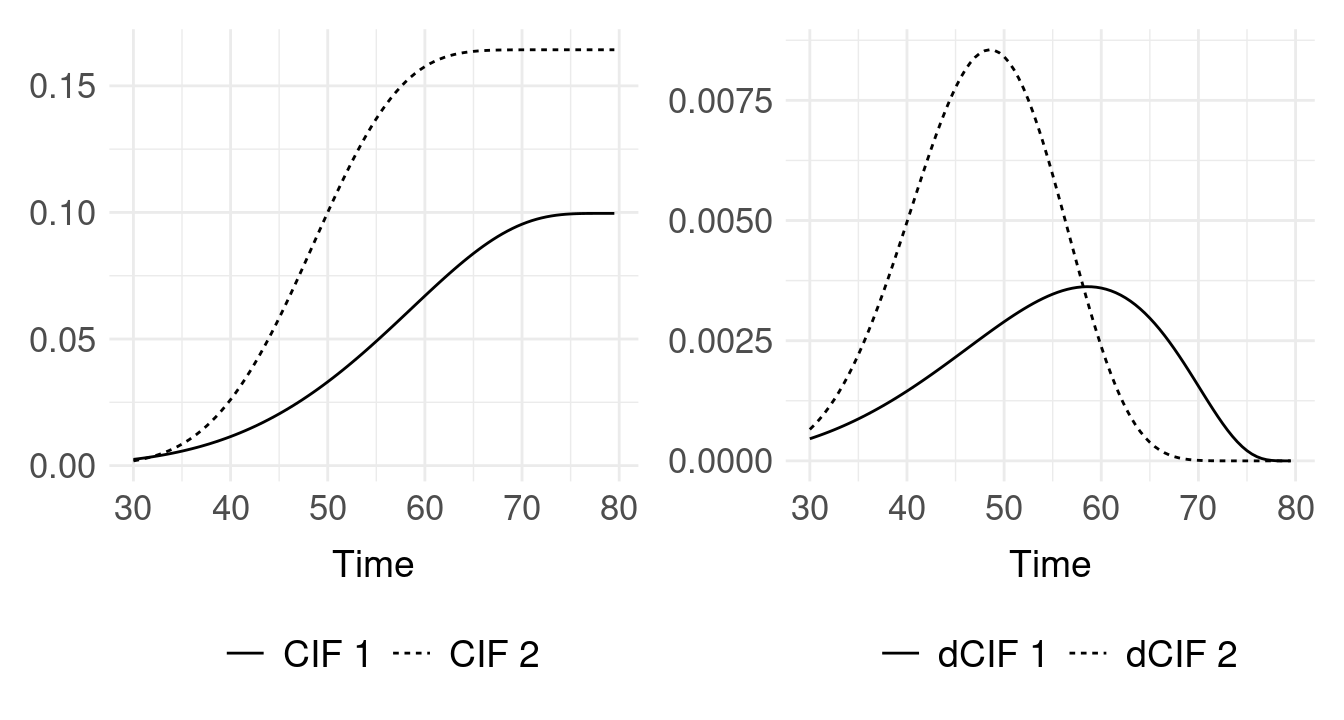
\includegraphics[width=\textwidth]{datasimucif-1.png}\\
 \begin{footnotesize}
  SOURCE: The author (2020).
 \end{footnotesize}
 \label{fig:datasimucif}
\end{figure}

By adding a complete latent structure,
\[
 \begin{bmatrix} u_{1}\\u_{2}\\\eta_{1}\\\eta_{2} \end{bmatrix}
 \sim\parbox{2.5cm}{\centering Multivariate Normal}
 \left(\begin{bmatrix} 0\\0\\0\\0 \end{bmatrix},
       \begin{bmatrix}
        1&0.4&0.5&0.4\\
         &1&0.4&0.3\\
         &&1&0.4\\
         &&&1
       \end{bmatrix}
 \right),
\]
we are able of apply Algorithm \autoref{alg:algo} to generate a complete
model sample with 500 clusters/pairs of twins, summarized in
\autoref{fig:datasimu}.

\begin{figure}[H]
  % \vspace{0.35cm}
  \setlength{\abovecaptionskip}{.0001pt}
  \caption{SUMMARY OF A SIMULATED DATASET WITH 500 PAIRS OF TWINS. A)
    TIME BY TWIN; B) TIMES BOXPLOT; C) PROBABILITIES SCATTERPLOT D)
    \(y_{3}\)'S \%}
  \vspace{0.2cm} \centering
  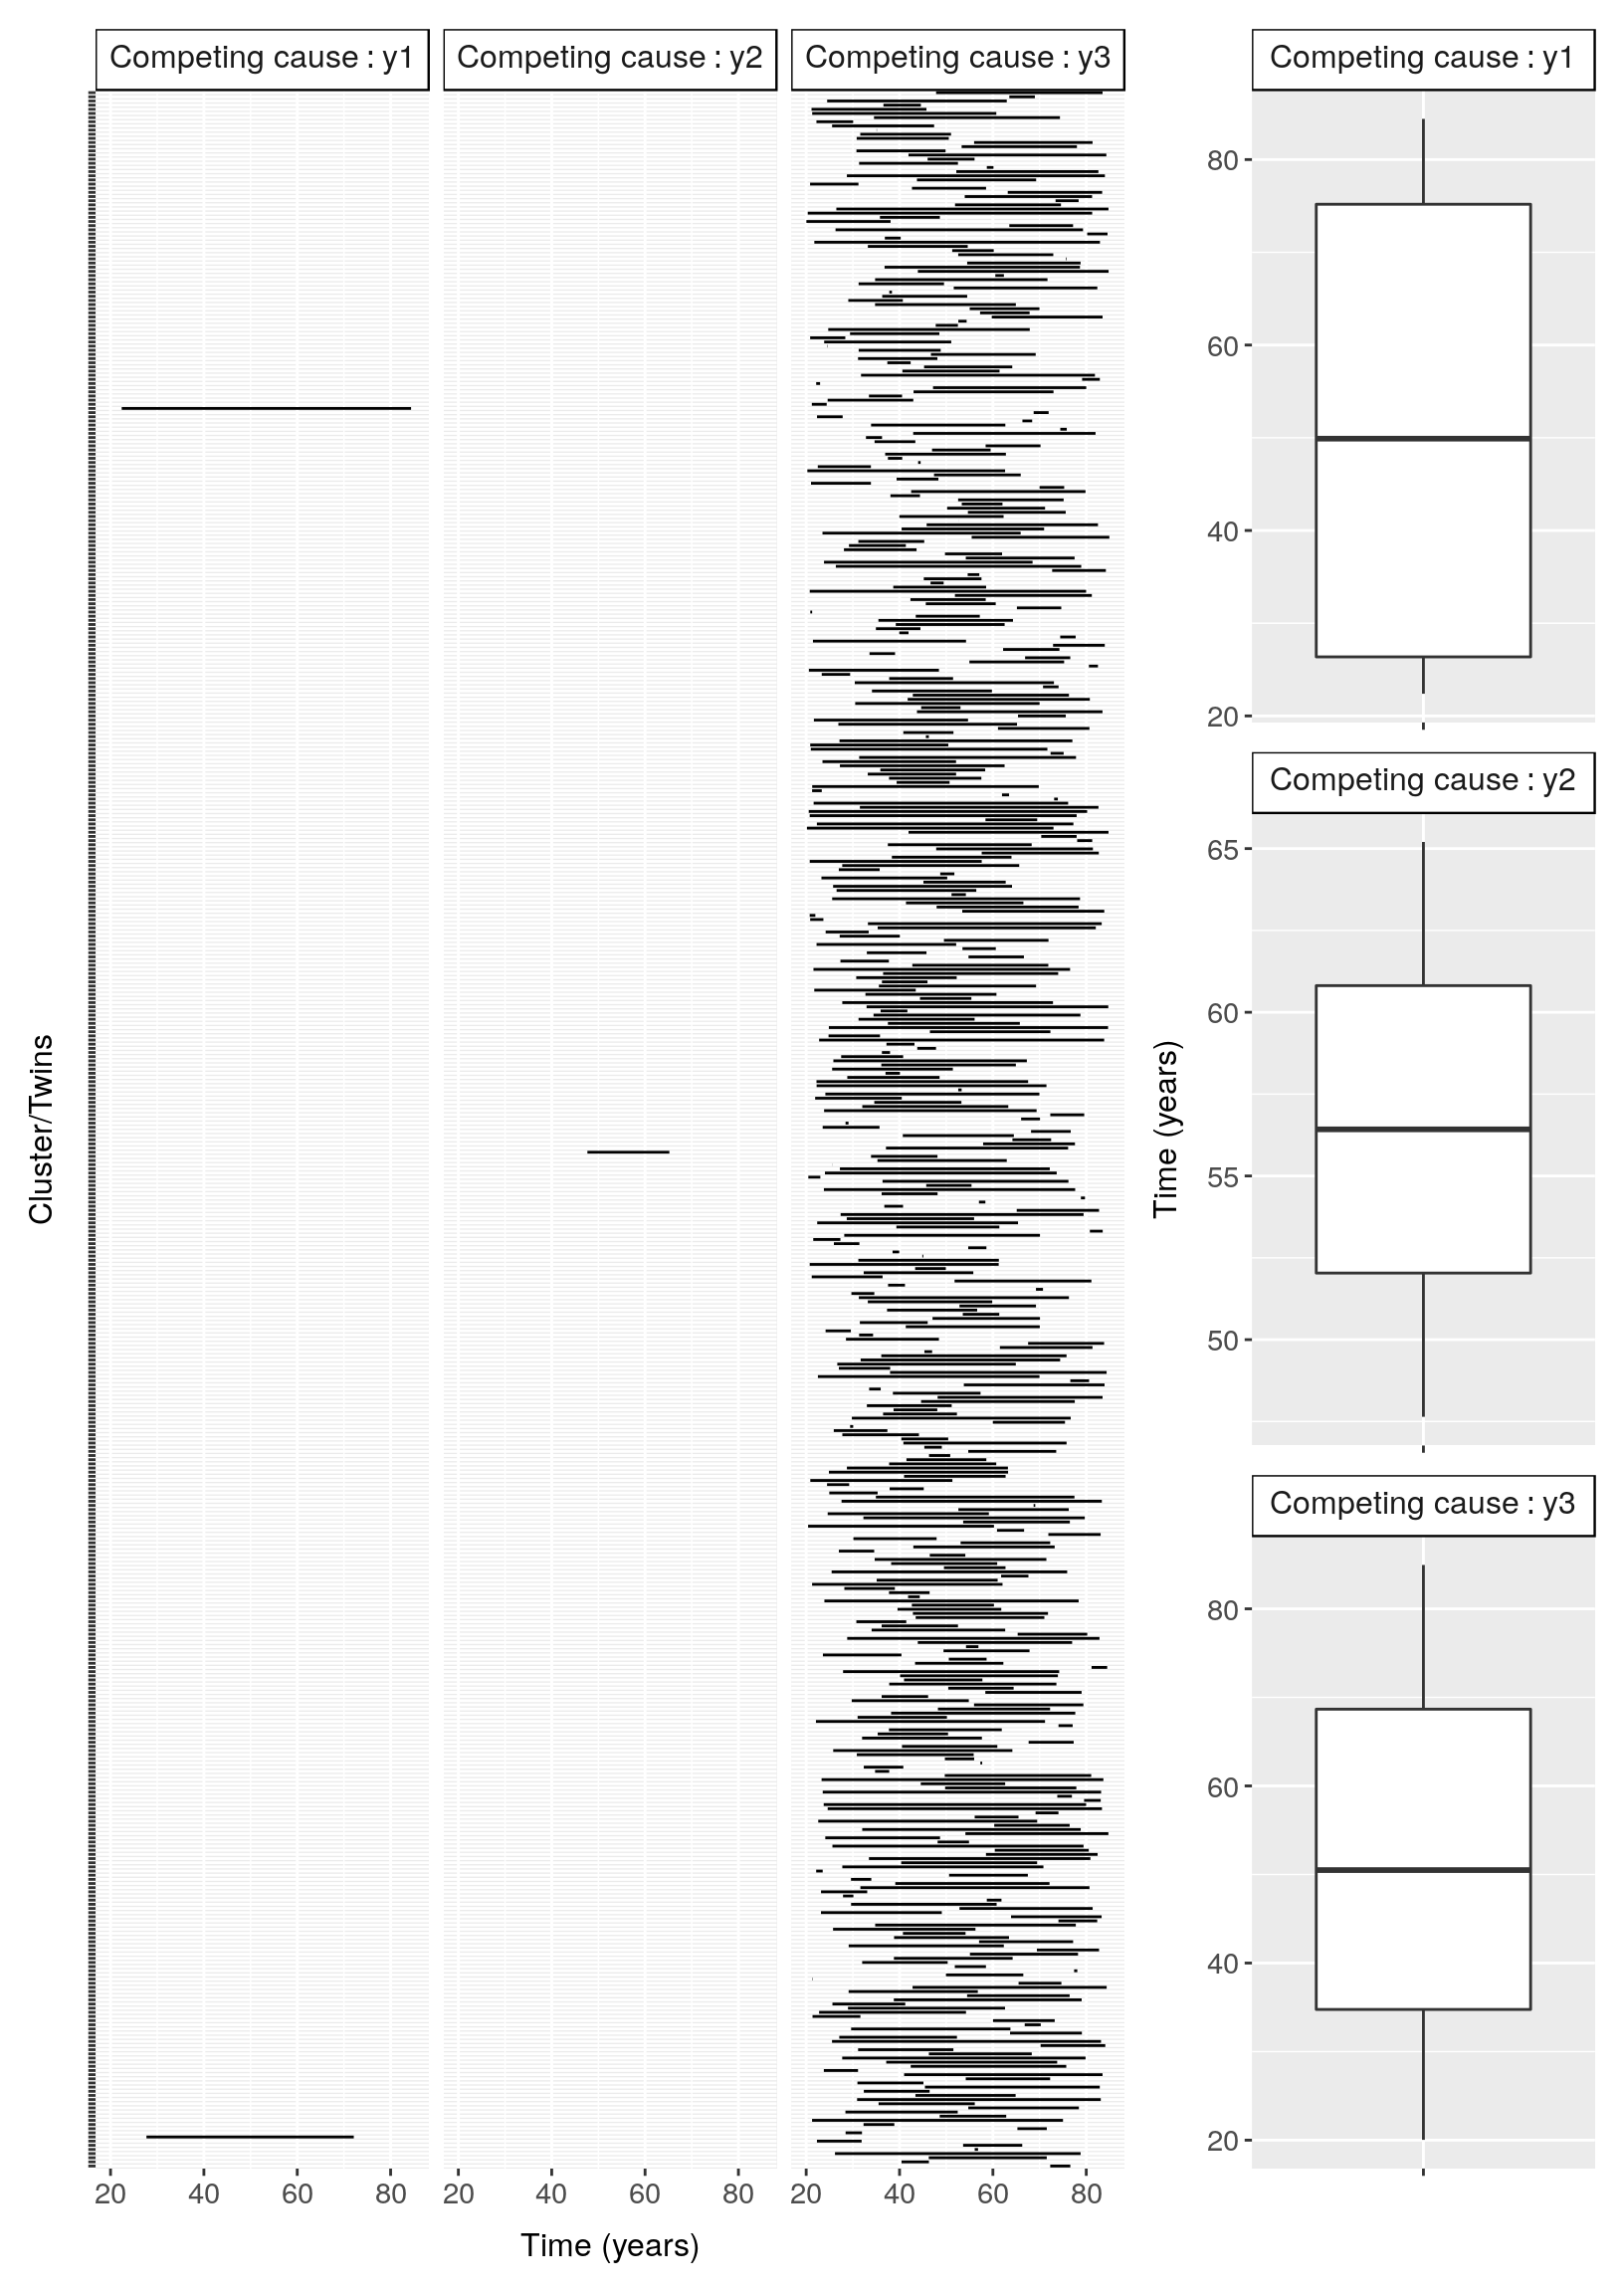
\includegraphics[width=\textwidth]{datasimu-1.png}
  \\
  \vspace{0.2cm}
  \begin{footnotesize}
    SOURCE: The author (2021).
  \end{footnotesize}
  \label{fig:datasimu}
\end{figure}

Sample \(\varsigma\sim\text{U}(0,~1)\)

Compute the cause-specific failure times by solving
\[
 \varsigma = \Phi[w_{k} g(t_{k}) - X^{\top}\gamma_{k} - \eta_{k}]
 \quad\text{for } t_{k}, \quad k = 1,~2,~\dots,~K - 1
\]

\section{REAL-BASED DATASET}
\label{cap:data}

% END ==================================================================
